\section{Entwicklung der Anwendung}\label{sec:entwicklung}

In Kapitel~\ref{sec:grundlagen} und~\ref{sec:architektur} wurden die notwendigen Grundlagen und die Architektur der Anwendung vermittelt.
Darauf aufbauend wird in den folgenden Abschnitten ein tieferer Einblick in die Entwicklungsphase gewährt und dazu passend Teile des Codes vorgestellt.
Daher ist dieses Kapitel in vier Abschnitte gegliedert, in denen jeweils eine Komponente der Anwendung behandelt wird.

\subsection{Erste Komponente: E-Graph}

Die Erstellung eines E-Graphs beginnt mit einem mathematischen Ausdruck, aus dem ein \textbf{Abstract Syntax Tree} (AST) aufgebaut wird.
Der AST wird später traversiert, um jeden Knoten dem E-Graph hinzuzufügen. Dieser Zwischenschritt vereinfacht die Erzeugung von E-Graphs und
kann gleichzeitig als Validierungsphase genutzt werden, da hier bereits feststeht, ob der Ausdruck der korrekten Form entspricht.

\subsubsection{AbstractSyntaxTree \& AbstractSyntaxTreeNode}

Ein AST erfordert die Klassen \textit{AbstractSyntaxTreeNode} (Listing~\ref{lst:astnode}) und 
\textit{AbstractSyntaxTree} (Listing~\ref{lst:ast}). Die Klasse \textit{AbstractSyntaxTreeNode} repräsentiert
einen Knoten im AST. Sie hat drei Attribute: eine linke Referenz, eine rechte Referenz und einen Schlüssel.

\begin{lstlisting}[language=Python, caption=Klasse \textit{AbstractSyntaxTreeNode}, label={lst:astnode}]
class AbstractSyntaxTreeNode:
    def __init__(self):
        self.left = None
        self.key = str()
        self.right = None
\end{lstlisting}

Der Schlüssel kann eine arithmetische Operation, eine Variable oder eine Zahl sein. Die Referenzen können auf einen weiteren Teilbaum, auf einen einzelnen Knoten
oder auf nichts zeigen. Mithilfe dieser Klasse kann nachher ein ganzer Baum dargestellt werden. Dazu muss lediglich der Wurzelknoten des Baumes abgespeichert werden, um über dessen Kinder
Zugriff auf den gesamten Baum zu erlangen. 

Durch die Klasse \textit{AbstractSyntaxTree} wird ein Ausdruck in einen AST transformiert. Sei der Ausdruck $(a \cdot 2) / 2$ als Beispiel gegeben.
Dieser muss von dem Benutzer zuerst in \textit{prefix}-Notation umgeschrieben werden. Dadurch entsteht der Ausdruck $(/\; (\cdot \;a \;2) \;2)$. Dies erleichtert die Transformation.
Entsprechend wird die Klasse mit diesem Ausdruck initialisiert, der durch die Methode \textit{\_process\_expression(self, expression)} verarbeitet wird.
\newpage

\begin{lstlisting}[language=Python, escapechar=|, caption=Auszug aus der Klasse \textit{AbstractSyntaxTree}, label={lst:ast}]
class AbstractSyntaxTree:
    # __init__, __str__ und _preorder weggelassen 

    def _process_expression(self, expression): |\label{astprocess}|
        root_ast_node = None
        stack = deque()
        word = ""
        for character in expression:
            if character == "(": |\label{ast0}|
                if not stack:
                    ast_node = AbstractSyntaxTreeNode()
                    stack.append(ast_node)
                    root_ast_node = ast_node
                else:
                    last_ast_node = stack[-1]
                    ast_node = AbstractSyntaxTreeNode()
                    # drei weitere Fälle, je nach Zustand des TOS
                    stack.append(ast_node)
            elif character in ("/", "*", "+", "-"): |\label{ast1}|
                last_ast_node = stack[-1]
                last_ast_node.key = character
            elif (word == "<" or word == ">") and (character == "<" or character == ">"): |\label{ast2}|
                word += character
                last_ast_node = stack[-1]
                last_ast_node.key = word
                word = ""
            elif (character == " " or character == ')') and word != "": |\label{ast3}|
                last_ast_node = stack[-1]
                # vier weitere Fälle, je nach Zustand des aktuellen TOS
                if character == ")":
                    stack.pop()
                word = ""
            elif character == ")" and word == "": |\label{ast4}|
                stack.pop()
            elif character == " ": |\label{ast5}|
                pass
            else: |\label{ast6}|
                word += character
        return root_ast_node
\end{lstlisting}

Die Methode~(Z. \ref{astprocess}) \textit{\_process\_expression} initialisiert drei lokale Variablen.
Die erste Variable \textit{root\_ast\_node} speichert den Wurzelknoten des Baumes, den die Methode später zurückgibt.
Die zweite Variable \textit{stack} speichert an der 
Position \textbf{Top of Stack} (TOS) den aktuell zu bearbeitenden Knoten. Die dritte Variable \textit{word} ist ein leerer String, der als kurzzeitiger Zwischenspeicher verwendet wird,
wenn Variablen, Zahlen oder Operationen aus mehreren Zeichen bestehen.
Der String wird von links nach rechts Zeichen für Zeichen verarbeitet, wobei sieben Fälle unterschieden werden.

\begin{wrapfigure}{r}{0.4\textwidth}
    %\vspace{-10mm}
    \begin{center}
      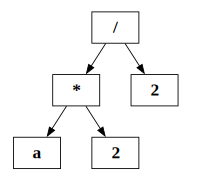
\includegraphics[scale=1.2]{../fig/ast.pdf}
    \end{center}
    \caption{Der AST für den Ausdruck $(a \cdot 2) / 2$}
    \label{fig:astexp}
\end{wrapfigure}

Fall eins~(Z.~\ref{ast0}) sorgt für die Erstellung eines neuen Knotens im Baum, da nach einer Klammer immer eine Operation folgt, die zwei Argumente hat.
Daher sorgt Fall zwei~(Z.~\ref{ast1}) dafür, dass der entsprechende Schlüssel dem letzten Knoten, der TOS ist, zugewiesen wird. 
Im dritten Fall~(Z.~\ref{ast2}) werden die beiden Shift-Operatoren ($<<, >>$) behandelt, die zwei Zeichen lang sind. Daher werden diese Operatoren separat behandelt und müssen
von dem Zwischenspeicher \textit{word} Gebrauch machen.
Im vierten Fall~(Z.~\ref{ast3}) werden Variablen und Zahlen verarbeitet und eventuell auch Knoten vom Stack genommen.
Fall fünf~(Z.~\ref{ast4}) behandelt einen ähnlichen Fall. Hierbei symbolisieren die schließende Klammer und der leere Zwischenspeicher, dass die Operation mit den zwei Argumenten abgeschlossen ist. 
Der sechste Falls~(Z. \ref{ast5}) wird nur behandelt, wenn das aktuelle Zeichen ein Leerzeichen ist. Diese werden übergangen.
Im siebten Fall~(Z.~\ref{ast6}) werden alle Variablen und Zahlen verarbeitet.

Nach der Beendigung der Methode gibt sie den Wurzelknoten des erstellten AST zurück, der im Attribut \textit{root\_node} der Klasse abgespeichert wird.
In Abbildung~\ref{fig:astexp} wird der fertige AST gezeigt.
Der \textit{ASTNode} mit dem Schlüssel $/$ fungiert dabei als \textit{root\_node}.
Die Klasse stellt weitere Methoden für eine Verifikation bereit, die den AST wieder in einen String transformieren. Dieser kann dann mit dem Original-String verglichen werden.

\subsubsection{E-Node}

Zur Umsetzung von E-Nodes wird eine weitere Klasse \textit{ENode} (Listing~\ref{lst:enode}) eingeführt. Dieses Vorgehen dient zur strikten Trennung der Komponenten.
Außerdem kann auf unnötige Attribute verzichtet werden. 
Der Klasse \textit{ENode} werden zwei Parameter übergeben: ein Schlüssel und eine Liste von EClass-IDs als Strings, die sie als ihre Attribute speichert.

\begin{lstlisting}[language=Python, caption=Klasse \textit{ENode}, label={lst:enode}]
class ENode:
    def __init__(self, key, arguments):
        self.key = key
        self.arguments = arguments
\end{lstlisting}

\subsubsection{E-Class}

Für die Erzeugung von E-Classes ist die Klasse \textit{EClass} (Listing~\ref{lst:eclass}) verantwortlich. 
Jede E-Class muss eindeutig identifizierbar sein, um eine E-Node der richtigen E-Class hinzufügen zu können.
Darüber hinaus ist es für das Mergen von E-Classes notwendig.
Für eine eindeutige Identifikation wird die Klasse mit einer UUID als ihre EClass-ID initialisiert. Dieser Ansatz stammt spezifisch aus~\cite{2021-egg}
und kann daher bei anderen Implementierungen variieren.

Weiterhin werden zwei Sets für E-Nodes und die Eltern der E-Class erzeugt.
Im Set für E-Nodes werden alle Knoten gespeichert, die Teil dieser Klasse sind.
Das Set mit Eltern der E-Class enthält Tuple. 
Jedes Tuple enthält eine E-Node $x$, die auf diese E-Class zeigt sowie die EClass-ID von $x$.
Die Referenzen auf Eltern der E-Class werden für den \textit{rebuild}-Schritt benötigt.

\begin{lstlisting}[language=Python, caption=Klasse \textit{EClass}, label={lst:eclass}]
# ... 

class EClass:
    def __init__(self):
        self.id = str(uuid.uuid4())
        self.nodes = set()
        self.parents = set()
\end{lstlisting}

\subsubsection{RewriteRule}

Die Klasse \textit{RewriteRule} (Listing~\ref{lst:rr}) dient als Repräsentant einer rewrite rule. Als Parameter bekommt sie einen Namen der Regel, einen linken sowie einen 
rechten Ausdruck übergeben. Die beiden Ausdrücke werden in ASTs umgewandelt. Die Attribute \textit{expr\_lhs} und \textit{expr\_rhs} speichern deshalb nur die Wurzelknoten der ASTs.

\begin{lstlisting}[language=Python, caption=Klasse \textit{RewriteRule}, label={lst:rr}]
# Importe ausgelassen 
class RewriteRule:
    def __init__(self, name, expr_lhs, expr_rhs):
        self.name = name
        self.expr_lhs = AbstractSyntaxTree(expr_lhs)
        self.expr_rhs = AbstractSyntaxTree(expr_rhs)

    # __str__ Methode weggelassen 
\end{lstlisting}

\subsubsection{EGraph}

Zusammen mit den bereits definierten Klassen kann anschließend die E-Graph-Datenstruktur angelegt werden. Dazu werden in der Init-Methode der Klasse \textit{EGraph} (Listing~\ref{lst:egraph})
die grundlegenden Datenstrukturen für einen E-Graph erstellt, wobei \textit{u} (Z.\ref{lst:union}) eine Union-Find-Datenstruktur ist.

\begin{lstlisting}[language=Python, escapechar=|, caption=Auszug aus der Klasse \textit{EGraph}, label={lst:egraph}]
# Importe ausgelassen 
class EGraph:
    def __init__(self):
        self.u = DisjointSet() |\label{lst:union}|
        self.m = {}
        self.h = {}
        self.pending = []
        self.version = 0
        self.str_repr = ""
        self.is_saturated = False
    # Methoden werden später behandelt
\end{lstlisting} 

\begin{wrapfigure}[24]{r}{0.6\textwidth}
\vspace{-7mm}
\hspace{3mm}
\begin{minipage}[t]{\linewidth}
\begin{lstlisting}[language=Python, escapechar=|, caption=Methoden der Klasse \textit{EGraph}, label={lst:methods1}]
def add_node(self, ast_root_node): |\label{lst:addnode}|
    # rekursiv Knoten des AST mit _add() zum E-Graph hinzufügen 

def _add(self, enode): |\label{lst:add}|
    enode = self._canonicalize(enode)
    # weitere Fälle 
    elif enode in self.h.keys(): |\label{lst:add1}|
        return self.h[enode]
    # weitere Fälle 
    else:
        self.version += 1
        eclass_id = self._new_singleton_eclass(enode)
        for child in enode.arguments:
            self.m[child].parents.add((enode, eclass_id)) |\label{lst:add2}|
        self.h[enode] = eclass_id
        return eclass_id

def _new_singleton_eclass(self, enode): |\label{lst:single}|
    # neue E-Class erstellen, enode hinzufügen
    
def _canonicalize(self, enode): |\label{lst:canonicalize}|
    return ENode(enode.key, [self._find(child) for child in enode.arguments])

def _find(self, eclass_id): |\label{lst:find}|
    return self.u.__getitem__(eclass_id)

def merge(self, eid1, eid2): |\label{lst:merge}|
    if self._find(eid1) == self._find(eid2):
        return self._find(eid1)
    self.version += 1
    self.u.merge(eid1, eid2) |\label{lst:merge1}|
    new_id = self._find(eid1) |\label{lst:merge2}|
    self.pending.append(new_id) |\label{lst:merge3}|
    return new_id
\end{lstlisting} 
\end{minipage}
\end{wrapfigure}

In Listing~\ref{lst:methods1} und~\ref{lst:methods2} werden acht Methoden aus~\cite{devito} definiert, die für die Basisfunktionalität eines E-Graphs notwendig sind.
Nachdem der Ausdruck in einen AST umgewandelt wurde, wird er der Methode \textit{add\_node} (Z.~\ref{lst:addnode}) übergeben. Die Methode erstellt eine E-Node aus dem Wurzelknoten
und fügt sie mit \textit{\_add} zum E-Graph hinzu. Die Argumente der E-Node entstehen durch das rekursive Aufrufen der Methode auf den Kindern des Wurzelknotens mit derselben Vorgehensweise.
Somit wird der gesamte AST dem E-Graph hinzugefügt.

Die Methode \textit{\_add} (Z.~\ref{lst:add}) ruft zuerst \textit{\_canonicalize} auf, weil der E-Graph geändert worden sein könnte.
\textit{\_canonicalize} (Z.~\ref{lst:canonicalize}) bildet aus der übergebenen E-Node die kanonische Form und gibt diese zurück.

Dafür wird wiederum die Methode \textit{\_find} (Z.~\ref{lst:find}) aufgerufen, die in der Union-Find-Datenstruktur den aktuellen Repräsentanten heraussucht.

Anschließend überprüft die \textit{\_add}-Methode, ob die E-Node in kanonischer Form bereits existiert (Z.~\ref{lst:add1}). Ist dies nicht der Fall, wird durch 
die Methode \textit{\_new\_singleton\_eclass} (Z.~\ref{lst:single}) eine neue E-Class erstellt, die E-Node hinzugefügt und in den E-Graph integriert. Dabei wird die E-Class zu den Eltern
ihrer Kinder hinzugefügt (Z.~\ref{lst:add2}). Dies ist für den \textit{rebuild}-Prozess wichtig.

Die Methode \textit{merge} vereinigt zwei E-Classes über ihre EClass-IDs. Dazu werden die Partitionen der Union-Find-Datenstruktur zusammengelegt (Z.~\ref{lst:merge1}) und ein (womöglich)
neuer Repräsentant bestimmt (Z.~\ref{lst:merge2}), der markiert wird (Z.~\ref{lst:merge3}). Die Markierung ist notwendig, damit im \textit{rebuild}-Schritt die Invarianten wiederhergestellt werden können.
Nach traditionellem Ansatz (siehe Kapitel~\ref{sec:grundlagen}) beinhaltet die \textit{merge}-Methode auch den \textit{rebuild}-Schritt. Die Entwickler von \textit{egg} konnten jedoch
zeigen, dass dieser Schritt ausgelagert werden kann~\cite{2021-egg}.

\begin{lstlisting}[language=Python, escapechar=|, caption=\textit{rebuild}- und \textit{repair}-Methode, label={lst:methods2}]
def rebuild(self): |\label{lst:rebuild}|
    for e_id in set([self._find(e_id) for e_id in self.pending]): |\label{lst:rebuild1}|
        self._repair(e_id)
    self.pending = []

def _repair(self, eclass_id): |\label{lst:repair}|
    for p_node, p_eclass in self.m[eclass_id].parents: |\label{lst:repair1}|
        if p_node in self.h.keys():
            self.h.pop(p_node)
        p_node = self._canonicalize(p_node)
        self.h[p_node] = self._find(p_eclass)
    new_parents = set()
    for p_node, p_eclass in self.m[eclass_id].parents: |\label{lst:repair2}|
        p_node = self._canonicalize(p_node)
        if p_node in [new_parent[0] for new_parent in new_parents]:
            for new_p_enode, new_p_eclass_id in new_parents:
                if new_p_enode == p_node: |\label{lst:repair3}|
                    self.merge(p_eclass, new_p_eclass_id) |\label{lst:repair4}|
        new_parents.add((p_node, self._find(p_eclass)))
    self.m[self._find(eclass_id)].parents = new_parents |\label{lst:repair99}|
\end{lstlisting} 

In der Methode \textit{\_rebuild} (Z.~\ref{lst:rebuild}) werden die EClass-IDs aus \textit{pending} zuerst durch ihre kanonische Form ersetzt. Ein Set vermeidet dabei Duplikate (Z.~\ref{lst:rebuild1}).  
Damit kann die Anzahl der \textit{\_repair}-Aufrufe reduziert werden.
Anschließend wird für jede EClass-ID die Methode \textit{\_repair} aufgerufen.

Bei dem \textit{Mergen} kann es vorkommen, dass die Eltern der E-Classes kongruent sind und daher ebenfalls gemerged werden müssen. Somit merged die Methode \textit{\_repair} (Z.~\ref{lst:repair}) 
rekursiv nach oben. Dafür werden zuerst die Eltern und deren Referenz auf die E-Class erneuert (Z.~\ref{lst:repair1}), da bei dem Merge-Vorgang zweier E-Classes eventuell ein anderer Repräsentant
gewählt wird. Dies führt dazu, dass die E-Nodes, die Eltern dieser E-Classes sind, eine falsche kanonische Form aufweisen.

Danach werden die Eltern neu festgelegt (Z.\ref{lst:repair2} bis \ref{lst:repair99}). Hierbei wird zuerst festgestellt, ob die Eltern bereits vorhanden sind (Z.\ref{lst:repair3}). Ist dies der Fall, werden sie
gemerged (Z.\ref{lst:repair4}).

\begin{lstlisting}[language=Python, escapechar=|, caption=\textit{apply\_rules}- und \textit{equality\_saturation}-Funktion, label={lst:methods3}]
def apply_rules(rules, egraph): |\label{lst:applyrules}|
    debug_info = []
    eclasses = egraph.get_eclasses()
    list_of_matches = []
    for rule in rules: |\label{lst:phase1}|
        for eclass_id, environment in egraph._ematch(eclasses, rule.expr_lhs.root_node):
            list_of_matches.append((rule, eclass_id, environment))
    for rule, eclass_id, environment in list_of_matches: |\label{lst:phase2}|
        new_eclass_id = egraph._substitute(rule.expr_rhs.root_node, environment)
        egraph.merge(eclass_id, new_eclass_id) |\label{lst:applymerge}|
    egraph.rebuild() |\label{lst:applyrebuild}|
    egraph.is_saturated = False
    return egraph, debug_info

def equality_saturation(rules, eterm_id, egraph): |\label{lst:eqsat}|
    debug_information = []
    best_term = ""
    timeout = 0
    if not egraph.is_saturated:
        # Verarbeitung der Debuginformationen
        while True and timeout < 5: |\label{lst:eqsat1}|
            v = egraph.version
            timeout += 1
            best_term = _extract_term(eterm_id, egraph) |\label{lst:extract}|
            # Verarbeitung der Debuginformationen
            egraph, debug = apply_rules(rules, egraph)
            # Verarbeitung der Debuginformationen
            if v == egraph.version:
                break
    return egraph, debug_information, best_term
\end{lstlisting} 

Nachdem die grundlegenden Methoden implementiert wurden, werden im Folgenden (Listing~\ref{lst:methods3}) zwei Funktionen aus~\cite{devito} eingeführt, mit deren Hilfe Equality Saturation durchgeführt werden kann.
Die Funktion \textit{apply\_rules} (Z.\ref{lst:applyrules}) ist für das Anwenden von rewrite rules auf den E-Graph verantwortlich. Der Vorgang kann in zwei Phasen unterteilt werden.
In der ersten Phase (Z.\ref{lst:phase1}) werden die rewrite rules herausgefiltert, deren linke Seite zu einem Teil des E-Graphs matchen. 
Die Funktion \textit{\_ematch()} iteriert über alle E-Classes und sucht dabei nach einem Muster, das zur linken Seite der Regel passt. Dabei entsteht eine Umgebung (\textit{environment}).
Das \textit{environment} ist eine Zuordnung von Variablen der linken Seite der Regel zu E-Classes, die für die Variablen infrage kommen. 

In der zweiten Phase (Z.\ref{lst:phase2})
wird mit der Methode \textit{\_substitute} die rechte Seite der Regel auf den E-Graph übertragen. Die Methode \textit{\_substitute} funktioniert auf ähnliche Weise wie die Funktion \textit{add\_node}.
Der übergebene AST wird rekursiv abgearbeitet, während die Knoten in E-Nodes umgewandelt und dem E-Graph mit \textit{\_add} hinzugefügt werden. Anschließend werden die neu erstellten E-Classes
mit den E-Classes aus dem environment gemerged (Z.~\ref{lst:applymerge}).
Nach den Phasen wird einmal \textit{rebuild} ausgeführt (Z.~\ref{lst:applyrebuild}). Wie im Paper~\cite{2021-egg} beschrieben, werden durch die \textit{merge}-Operationen kurzzeitig die Invarianten verletzt, 
die aber zum Schluss von \textit{apply\_rules} wiederhergestellt werden.

Die Funktion \textit{equality\_saturation} (Z.\ref{lst:eqsat}) ist für das Verfahren der Equality Saturation zuständig. Um den E-Graph zu saturieren, werden solange Regeln angewendet, bis
dieser saturiert oder ein Timeout erreicht wird (Z.~\ref{lst:eqsat1}).
Das Timeout ist notwendig, da im Falle eines Zyklus im E-Graph (siehe Kapitel~\ref{sec:reflexion}) eine Endlosschleife ausgeführt wird.
Während der Ausführung wird ein optimaler Ausdruck aus dem E-Graph mit \textit{\_extract\_term} extrahiert (Z.~\ref{lst:extract}).
Die Funktion \textit{\_extract\_term} berechnet auf der Grundlage eines einfachen Kostenmodelles: Jede E-Node kostet so viel wie die Summe ihrer Kinder, zuzüglich ihrer Kosten.
Dabei erhalten E-Nodes ohne Operationen Kosten von null. E-Nodes mit Addition, Subtraktion oder Shift-Operationen
erhalten Kosten von eins, E-Nodes mit Multiplikation erhalten Kosten von zwei und E-Nodes mit Division erhalten Kosten von drei.
Durch diese Berechnung kann der günstigste (optimale) Ausdruck aus dem E-Graph extrahiert werden.

\begin{lstlisting}[language=Python, escapechar=|, caption=\textit{egraph\_to\_dot}-Methode, label={lst:methods4}]
def egraph_to_dot(self, nodesep=0.5, ranksep=0.5, marked_eclasses = []):
    dot_commands = [
        # String, der Graph in DOT-Format anlegt
    ]
    node_set = set()
    node_identifier = 0
    for subset in self.u.subsets(): |\label{lst:dot1}|
        # wenn E-Class in marked_eclasses, dann fillcolor=crimson
        dot_commands.append(
            # subgraph wird als cluster hinzugefügt
        )
        nodes_in_subset = set()
        for eclass_id in subset: |\label{lst:dot11}|
            for n in self.m[eclass_id].nodes:
                nodes_in_subset.add(n)

        for enode in nodes_in_subset: |\label{lst:dot12}|
            # berechne Nummer
            node_set.add(
                (str(self._find(next(iter(subset)))), node_identifier, enode)
            )
            second_diff = enode.key
            if enode.key in ('<<', '>>'): |\label{lst:dot13}|
                second_diff = enode.key[0] + '\\' + enode.key[1]
            dot_commands.append(
                # enode wird zum subgraph hinzufügt
            )
            node_identifier += 1 |\label{lst:dot14}|
        dot_commands.append("}\n") |\label{lst:dot2}|

    for ecl_id, node_ident, enode in node_set: |\label{lst:dot3}|
        if enode.arguments:
            # lokale Variablen werden angelegt
            enode_arg0, enode_arg1 = enode.arguments
            k0 = next(iter(self.m[enode_arg0].nodes))
            k1 = next(iter(self.m[enode_arg1].nodes))
            # wenn k0 oder k1 Operation, dann berechne linke und rechte Nummer 

            if self._find(enode_arg0) == ecl_id: |\label{lst:dot31}|
                dot_commands.append(
                    # E-Node zeigt auf eigene E-Class
                )
            else:
                dot_commands.append(
                    # E-Node zeigt auf E-Class
                ) |\label{lst:dot32}|

            if self._find(enode_arg1) == ecl_id: |\label{lst:dot33}|
                dot_commands.append(
                    # E-Node zeigt auf eigene E-Class
                )
            else:
                dot_commands.append(
                    # E-Node zeigt auf E-Class 
                ) |\label{lst:dot4}|
    dot_commands.append("}")
    return "".join(dot_commands) |\label{lst:dot5}|  
\end{lstlisting} 

In Listing~\ref{lst:methods4} wird die Methode \textit{egraph\_to\_dot} zur Visualisierung eines E-Graphs dargestellt. Die Vorgehensweise wird in zwei Phasen unterteilt.
In der ersten Phase (Z.~\ref{lst:dot1} bis~Z.~\ref{lst:dot2}) wird für jede Partition der Union-Find-Datenstruktur ein \textit{subgraph} erstellt. Dabei werden aus allen
E-Classes der Partition die E-Nodes herausgefiltert (Z.~\ref{lst:dot11}). Anschließend wird für jede E-Node eine \textit{Node} erzeugt (Z.~\ref{lst:dot12}).
Wenn die E-Node eine Shift-Operation als Schlüssel enthält, muss die Operation \textit{escaped} werden (Z.~\ref{lst:dot13}).
Zum Schluss der Schleife muss der \textit{node\_identifier} aktualisiert werden (Z.~\ref{lst:dot14}). Dies liegt daran, dass die \textit{Nodes} im DOT-Format
jeweils einen linken und rechten Pfeil haben und diese separat angesprochen werden müssen.

In der zweiten Phase (Z.~\ref{lst:dot3} bis~Z.~\ref{lst:dot4}) werden die Pfeile gezeichnet. 
Hierbei wird für jedes Argument der E-Node separater Code ausgeführt (Z.~\ref{lst:dot31} bis~Z.~\ref{lst:dot32} und Z.~\ref{lst:dot33} bis~Z.~\ref{lst:dot4}).
Zusätzlich muss für jedes Argument der Fall eines Zyklus im E-Graph unterstützt werden (Z.~\ref{lst:dot31} und Z.~\ref{lst:dot33}).
Schließlich werden die einzelnen Strings zu einem zusammengefügt und zurückgegeben (Z.~\ref{lst:dot5}). 

\subsection{Zweite Komponente: Service}

Während der Server Anfragen der Benutzeroberfläche beantwortet, regelt der Service im Hintergrund die Erstellung und Verwaltung von E-Graphs.
Die schrittweise Darstellung von Veränderungen des E-Graphs stellt das Kernstück der Anwendung dar. 
Da die meisten anderen Funktionen des Service auch ohne Erklärung verstanden werden können, wird dieses Feature in den folgenden Abschnitten bevorzugt behandelt.
Der Service wurde in der Klasse \textit{EGraphService} implementiert. Die Initialisierung der Klasse erfolgt in Listing~\ref{lst:serviceinit}.

\begin{lstlisting}[language=Python, escapechar=|, caption=Auszug aus der Datei \textit{EGraphService.py}, label={lst:serviceinit}]
# Importe und is_valid_expression(expression) ausgelassen 

class EGraphService:
    def __init__(self):
        self.rrc = 0
        self.dict_of_rules = {}
        self.applied_rules = set()
        self.egraph = None
        self.expr = None
        self.egraphs = [[]] |\label{lst:serviceegraphs}|
        self.current_major = 0
        self.current_minor = 0

# weitere Methoden weggelassen
\end{lstlisting} 

Darauf aufbauend bilden die vier Methoden in Listing~\ref{lst:servicemove} die Grundlage des Debugging-Features.

\begin{lstlisting}[language=Python, escapechar=|, caption=Methoden für das Debugging aus der Datei \textit{EGraphService.py}, label={lst:servicemove}]
def move_backward(self):
    if self.current_minor == 0:
        if self.current_major == 0:
            pass # ganz hinten angekommen
        else:
            self.current_major -= 1
            self.current_minor = len(self.egraphs[self.current_major]) - 1
    else:
        self.current_minor -= 1

def move_forward(self):
    if len(self.egraphs[self.current_major]) - 1 == self.current_minor:
        if self.current_major == len(self.egraphs) - 1:
            pass # ganz vorne angekommen
        else:
            self.current_minor = 0   # am Ende dieser Liste angekommen,
            self.current_major += 1  # beim Anfang der nächsten starten
    else:
        self.current_minor += 1

def move_fastbackward(self):
    if self.current_major != 0:
        self.current_major -= 1
        self.current_minor = len(self.egraphs[self.current_major]) - 1
        # ^- letzte Änderung am Ende der Liste, daher dorthin springen

def move_fastforward(self):
    if self.current_major != len(self.egraphs) - 1:
        self.current_major += 1
        self.current_minor = len(self.egraphs[self.current_major]) - 1
        # ^- letzte Änderung am Ende der Liste, daher dorthin springen
\end{lstlisting} 

Das Debugging-Feature beruht auf folgender Idee: Der Service speichert eine Liste mit Änderungen, die am E-Graph durchgeführt worden sind.
Dazu wird bei jeder Änderung ein Abbild des E-Graphs im DOT-Format erstellt.
Möchte der Nutzer eine Änderung erneut begutachten, kann er in der Liste zurückspringen. Um feinere Details abspeichern zu können, wird 
eine Änderung in mehrere kleine Änderungen zerlegt, die alle in einer Liste gespeichert werden. Dies resultiert in einer Liste von Listen,
die im Attribut \textit{self.egraphs} gespeichert wird (Listing~\ref{lst:serviceinit}, Z.~\ref{lst:serviceegraphs}).

Die beiden Methoden \textit{move\_forward} und \textit{move\_backward} (Listing~\ref{lst:servicemove}) regeln das Vor- und Zurückspringen innerhalb einer Liste mit kleinen Änderungen.
Die anderen beiden Methoden \textit{move\_fastforward} und \textit{move\_fastbackward} regeln den Sprung von Änderung zu Änderung.
Für die Position innerhalb der Listen gibt es zwei Attribute: \textit{self.current\_minor} und \textit{self.current\_major}. Mit \textit{self.current\_major} kann von Änderung
zu Änderung gesprungen werden, während \textit{self.current\_minor} innerhalb der Änderung vor- oder zurückspringt.

Diese Vorgehensweise ermöglicht es, das Abbild des E-Graphs im DOT-Formatan der Position \textit{self.egraphs[self.current\_major][self.current\_minor]} abzufragen,
das durch den Server an die Benutzeroberfläche geschickt und dort gerendert wird.

\subsection{Dritte Komponente: Server}

Als dritte Komponente der Anwendung ermöglicht der Server die Kommunikation zwischen Service und Weboberfläche. 
Die Datei \textit{server.py} (Listing~\ref{lst:server}) enthält den Server, der mit dem Framework FastAPI realisiert wurde.

\noindent Zu Beginn werden zwei Instanzen initialisiert. Die erste Instanz ist der Server selbst (Z.~\ref{serverinit}), die zweite der EGraphService (Z.~\ref{serverservice}).
Der Serverinstanz wird die Funktion \textit{lifespan} übergeben, die bei dem Starten und Herunterfahren des Servers benutzerdefinierte Aktionen ausführen kann.
In diesem Fall wird der Browser unter der Adresse \url{http://127.0.0.1:8000} geöffnet (Z.~\ref{serveropen}).

\begin{lstlisting}[language=Python, escapechar=|, caption=Auszug aus der Datei \textit{server.py}, label={lst:server}]
# Importe ausgelassen 

@asynccontextmanager
async def lifespan(app: FastAPI):
    open_new(r"http://127.0.0.1:8000") |\label{serveropen}|
    yield

app = FastAPI(lifespan=lifespan) |\label{serverinit}|
egraphService = EGraphService() |\label{serverservice}|

# Funktion get_rules() weggelassen

@app.post("/addrule") |\label{serverendpoint}|
async def add_rule(request: Request): |\label{serverrequestbody}|
    payload = await request.body() |\label{serverawait}|
    data = json.loads(payload) |\label{serverjson}|
    result, msg = egraphService.add_rule(data["lhs"], data["rhs"]) |\label{serveraction}|
    return {"response": str(result), "msg": msg} |\label{serverresponse}|

# weitere Funktionen für mehr Übersichtlichkeit weggelassen 

app.mount("/", StaticFiles(directory=realpath(f"{realpath(__file__)}/../static"), html=True), name="static") |\label{serverend}|
\end{lstlisting} 

Nach der Initialisierung der Instanzen folgen die Endpunkte bzw. Pfadoperationen, die der Benutzeroberfläche durch den Server zur Verfügung gestellt werden.
Am Beispiel der Funktion \textit{add\_rule} (Z.~\ref{serverendpoint}) soll der typische Aufbau eines Endpunktes erläutert werden.

Als Erstes wird die Funktion mit der HTTP-Methode \textit{post} annotiert, die auch den Pfad enthält (Z.~\ref{serverendpoint}).
Dadurch wird festgelegt, welche Struktur eine Anfrage haben muss.
Als Zweites folgt die Funktionsdefinition (Z.~\ref{serverrequestbody}). Dabei wird ein \textit{Request} erwartet (Z.~\ref{serverawait}), der die entsprechenden Daten enthält. 
Die JSON-Daten aus dem Request werden danach in ein Dictionary umgewandelt (Z.~\ref{serverjson}).
Im Anschluss daran werden die Daten an den Service übergeben, der diese auf Korrektheit überprüft und sie dem Service hinzufügt (Z.~\ref{serveraction}).
Zum Schluss wird eine Response im JSON-Format an die Benutzeroberfläche zurückgegeben (Z.~\ref{serverresponse}).

Die letzte Anweisung in der Datei (Z.~\ref{serverend}) dient dazu, alle Dateien im Ordner \textit{static/} unter dem Pfad \textit{/} freizugeben, ohne jeweils Endpunkte einrichten zu müssen.
Der Ordner enthält die Benutzeroberfläche als HTML-Dokument und weitere Hilfsdateien. Somit kann die Benutzeroberfläche direkt unter der Adresse \url{http://127.0.0.1:8000/}
aufgerufen werden. Um die vorher definierten Pfadoperationen nicht zu verdecken, muss diese Anweisung am Ende der Datei stehen.
Die Angabe des Pfades erfolgt durch \textit{realpath}, da es sonst zu Problemen mit den Tests gekommen wäre (siehe Kapitel~\ref{sec:probleme}).

\subsection{Vierte Komponente: Weboberfläche}

Die vierte Komponente besteht aus einer Benutzeroberfläche mit Dokumentation und dem dazugehörigen JavaScript-Code, der für die Funktionalität und Kommunikation mit dem Server
zuständig ist.

\subsubsection{Benutzeroberfläche und Dokumentation}

Die Benutzeroberfläche (Abbildung~\ref{fig:website}) startet mit einer Navigation ganz oben auf der Website. Über die angegebenen Links können die Dokumentation (Abbildung~\ref{fig:docs}) und die About-Seite aufgerufen werden.
Darunter ist die Anwendung in drei Segmente unterteilt. Das erste Segment ist für die Visualisierung von E-Graphs verantwortlich. Das zweite Segment ist für rewrite rules zuständig, während das dritte Segment
die Erstellung von E-Graphs und weitere Steuerungselemente beinhaltet.

\newpage
\begin{figure}[H]
\centering
\includegraphics[scale=0.42, angle=90]{../fig/website.png}
\caption{Website der Anwendung}
\label{fig:website}
\end{figure}
\newpage

\begin{figure}[H]
\centering
\includegraphics[scale=0.42, angle=90]{../fig/docs.png}
\caption{Dokumentation der Anwendung, Abschnitt Installation}
\label{fig:docs}
\end{figure}
\newpage

\begin{figure}[H]
    \centering
    \includegraphics[scale=0.5]{../fig/egraphcontrol.png}
    \caption{Segment zur Darstellung von E-Graphs}
    \label{fig:segment1}
\end{figure}

Im ersten Segment (Abbildung~\ref{fig:segment1}) wird der E-Graph als SVG gerendert. Durch Bewegung des Mausrades oder Benutzung des Touchpads kann die Darstellung vergrößert und verkleinert werden.
Der Cursor ermöglicht das Verschieben der Darstellung innerhalb des hellgrauen Kastens. Hovert der Benutzer länger über einer beigen E-Class, wird ihre EClass-ID angezeigt.
Zusätzlich verfügt das Segment über den Link \textit{Open in new tab}, durch den
sich ein neuer Tab mit einer größeren Darstellung des E-Graphs öffnet. Dadurch werden Probleme mit der variierenden Bildschirmgröße von Nutzern umgangen.

\begin{wrapfigure}[16]{r}{0.5\textwidth}
    \vspace{-10mm}
    \begin{center}
      \includegraphics[scale=0.6]{../fig/rewriterulecontrol.png}
    \end{center}
    \caption{Segment für rewrite rules}
    \label{fig:segment2}
\end{wrapfigure}

Das zweite Segment (Abbildung~\ref{fig:segment2}) besteht aus drei Untersegmenten, die Erstellung, Sicherung und Anwendung von \textit{rewrite rules} regeln. 
Dabei minimiert der schwarze Pfeil in der rechten oberen Ecke dieses Segment und sorgt bei schmaleren Bildschirmen für eine effizientere Aufteilung des Inhalts.
Das erste Untersegment \textbf{Create} besteht aus zwei Eingabefeldern und einem Button \textit{Create}, durch die der Benutzer eine Regel eingeben und abschicken kann.
Im zweiten Untersegment \textbf{Rules} können die Regeln, die zu diesem Zeitpunkt in der Anwendung abgespeichert sind, mit dem \textit{Download}-Button in einer Datei gesichert werden.

Nach einem Neustart der Anwendung können diese durch den \textit{Upload}-Button automatisch wieder zur Anwendung hinzugefügt werden. 

Im dritten Untersegment werden alle Regeln aufgelistet. Möchte der Benutzer eine oder mehrere Regeln anwenden, können diese durch die Checkboxen ausgewählt und durch den 
Button \textit{Apply} auf den E-Graph angewendet werden. Der Button \textit{Saturate} führt eine Saturierung des E-Graphs durch, indem alle Regeln solange auf den E-Graph angewendet werden, bis sich keine Änderungen mehr ergeben.

\begin{wrapfigure}{r}{0.5\textwidth}
    \vspace{-10mm}
    \begin{center}
      \includegraphics[scale=0.6]{../fig/control1.png}
    \end{center}
    \caption{Kontrollsegment, Teil 1}
    \label{fig:segment31}
\end{wrapfigure}

Im dritten Segment (Abbildung~\ref{fig:segment31} und Abbildung~\ref{fig:segment32}) befinden sich eine Funktion zur Erstellung von E-Graphs sowie weitere Steuerungselemente für die Anwendung.
Im oberen Teil des Segments wurden drei Untersegmente platziert. Im ersten Untersegment \textbf{Create} kann durch die Eingabe eines Terms und die Betätigung des \textit{Create}-Buttons
ein E-Graph erzeugt werden. Das zweite Untersegment \textbf{Debug} zeichnet sich durch zwei Radio-Buttons (\textit{Standard} und \textit{Debug}) sowie vier weitere Buttons aus. 

Durch die Radio-Buttons kann der Benutzer zwischen der Standardausgabe (\textit{Standard}) und einer detaillierten Debugausgabe (\textit{Debug}) wählen.
Mit den vier Buttons unterhalb der Radio-Buttons kann durch die Ausgabe gesprungen werden. Die beiden Buttons \textbf{<<} und \textbf{>>} zeigen den E-Graph jeweils nach oder vor einer 
Reihe von Änderungen. Durch die anderen zwei Buttons (\textbf{<} und \textbf{>}), die nur im Debug-Modus aktiviert sind, kann der Benutzer jede einzelne Änderung am E-Graph verfolgen. 

In dem dritten Untersegment \textbf{Extract} kann durch die Betätigung des \textit{Extract}-Buttons der optimale Ausdruck aus dem E-Graph extrahiert und in dem darüber liegenden grauen Feld angezeigt werden.
Die Prozedur der Extraktion kann danach im Debug-Modus detailliert beobachtet werden. 
Der Benutzer kann den \textit{Best Term}-Button betätigen, um den optimalen Ausdruck zu kopieren.
\newpage

\begin{wrapfigure}{r}{0.5\textwidth}
    \vspace{-5mm}
    \begin{center}
      \includegraphics[scale=0.6]{../fig/control2.png}
    \end{center}
    \caption{Kontrollsegment, Teil 2}
    \label{fig:segment32}
\end{wrapfigure}

Im unteren Teil des dritten Segments (Abbildung~\ref{fig:segment32}) befinden sich drei weitere Untersegmente.  
Das erste Untersegment \textbf{Export} stellt dem Benutzer drei mögliche Formate (PDF, SVG und PNF) für den Export des E-Graphs zur Verfügung. Durch die Betätigung des \textit{Export}-Buttons
wird der E-Graph in das ausgewählte Dateiformat exportiert.
Das zweite Untersegment \textbf{Session} ermöglicht dem Benutzer, durch Drücken des \textit{Download}-Buttons seine Sitzung als Datei zu sichern. Zudem kann die Sitzung bei Bedarf
durch den \textit{Upload}-Button wiederhergestellt werden. 
In der Sitzungsdatei wird der Ausdruck gespeichert, durch den der E-Graph erstellt wurde. 
Zudem werden eine Liste der rewrite rules sowie eine Kennzeichnung, welche der Regeln bereits auf den E-Graph angewendet wurden, gespeichert.
Darüber hinaus enthält die Sitzungsdatei den eventuell extrahierten, optimalen Ausdruck.
Das dritte Untersegment \textbf{Status} ist eine Liste mit Informationen, Warnungen und Fehlern, die dem Benutzer als Rückmeldung dienen. Wenn der Benutzer die Änderungen am E-Graph beobachtet, werden
darüber hinaus Debug-Informationen angezeigt. Werden zwei E-Classes gemerged, wird in der Statusleiste angezeigt, um welche E-Classes es sich handelt.  

\subsubsection{JavaScript}

JavaScript regelt die Manipulation der Benutzeroberfläche und die Kommunikation mit dem Server. Im Folgenden werden die Abläufe während der Kommunikation näher erläutert.

Die Kommunikation mit dem Server wird durch die Funktion \textit{contactServer} möglich (Listing~\ref{lst:js}).
Der Funktion werden drei Parameter übergeben (Z.~\ref{js:a1}): ein String für die Route (\textit{path}), zum Beispiel /add\_rule, Daten im JSON-Format (\textit{payload})
und die HTTP-Methode (\textit{httpMethod}). In den Zeilen~\ref{js:a2} bis~\ref{js:a3} wird aus den Parametern ein neuer Request vorbereitet. Sollte dabei kein \textit{payload}
angegeben werden (Z.~\ref{js:a21}), wird kein \textit{payload} mitgeschickt. Der vorbereitete Request wird in Zeile~\ref{js:return} an den Server geschickt. Dabei wird mit \textit{await}
die Ausführung pausiert, bis eine Antwort erhalten wurde. Dies funktioniert nur in einer asynchronen Funktion, weshalb \textit{contactServer} entsprechend mit \textit{async} 
markiert wurde (Z.~\ref{js:a1}). Die Antwort wird in das JSON-Format umgewandelt und zurückgegeben (Z.~\ref{js:return}).

\begin{lstlisting}[language=JavaScript, escapechar=|, caption=Auszug aus der Datei \textit{index.js}, label={lst:js}]
async function contactServer(path, payload, httpMethod) { |\label{js:a1}|
    let request; |\label{js:a2}|
    if (payload == null) { |\label{js:a21}|
        request = new Request("http://127.0.0.1:8000" + path, {
            method: httpMethod
        });
    } else {
        request = new Request("http://127.0.0.1:8000" + path, {
            method: httpMethod,
            body: payload,
        });
    } |\label{js:a3}|
    return (await fetch(request)).json(); |\label{js:return}|
}
\end{lstlisting} 

Dieser Ablauf wird im Folgenden anhand eines Beispiels verdeutlicht.
Bei dem Anlegen einer neuen rewrite rule wird durch die Betätigung des Buttons \textit{Apply} die Funktion \textit{applyRewriteRules} ausgeführt (Listing~\ref{lst:apply}).

Die Funktion startet mit einer Sammlung der vom Benutzer ausgewählten Regeln in einem Array (Z.~\ref{js:b1} -~\ref{js:b2}, hier nicht gezeigt).
Im zweiten Schritt wird \textit{contactServer} mit den Parametern aufgerufen (Z.~\ref{js:b3} -~\ref{js:b4}).
Die Funktion \textit{contactServer} liefert dabei die Daten im JSON-Format zurück, die durch die asynchrone Eigenschaft der Funktion automatisch in ein \textit{Promise}-Objekt gewrapped werden (Z.~\ref{js:b4}).
Ein \textit{Promise}-Objekt stellt das Ergebnis einer asynchronen Funktion dar~\footnote{\hspace{1.5mm}\url{https://developer.mozilla.org/de/docs/Web/JavaScript/Reference/Global_Objects/Promise}}.
Eine Funktion kann erfolgreich ausgeführt werden (Z.~\ref{js:b5}) oder fehlschlagen (Z.~\ref{js:b6}). Im ersten Fall wird, basierend darauf, ob der Benutzer überhaupt eine Regel ausgewählt hat,
eine Warnung (Z.~\ref{js:b8}) oder eine Bestätigung (Z.~\ref{js:b9}) als Statusmeldung angezeigt.
Im zweiten Fall wird eine Fehlermeldung angezeigt (Z.~\ref{js:b7}), wenn der Request fehlschlägt.

\begin{lstlisting}[language=JavaScript, escapechar=|, caption=Funktion \textit{applyRewriteRules()} aus der Datei \textit{index.js}, label={lst:apply}]
function applyRewriteRules() {
    let rrNumbers = []; |\label{js:b1}|
    // Filtere die ausgewählten Regeln heraus und füge sie in rrNumbers ein
    //... |\label{js:b2}|
    contactServer("/applyrule", |\label{js:b3}|
        JSON.stringify({"payload": rrNumbers}), "POST").then( |\label{js:b4}|
        function (value) { |\label{js:b5}|
            if (value['response'] === "False") {
                addMessageToStatusBar("[WARN]", value['msg']); |\label{js:b8}|
            } else {
                addMessageToStatusBar("[INFO]", value['msg']); |\label{js:b9}|
            }
        }, function () { |\label{js:b6}|
            addMessageToStatusBar("[ERROR]", "Failed to contact server."); |\label{js:b7}|
        }); 
}
\end{lstlisting} 
